\documentclass{./../handout}
% Sections & Subsections
\usepackage{sectsty}
\renewcommand{\thesection}{\arabic{section}} 
\renewcommand{\thesubsection}{\arabic{section}.\arabic{subsection}} 
  \sectionfont{\large \normalfont \sc}
\subsectionfont{\fontsize{13}{1} \normalfont \textit}
\subsubsectionfont{\fontsize{12}{1} \normalfont \textit}

\fancyhf{}
\lhead{ECON 340: Economic Research Methods}
\rhead{Div Bhagia}
\rfoot{\center \thepage}

\begin{document}
\thispagestyle{plain}
\begin{center}
  \framebox{
    \vbox{
    \vspace{1em}
     \Large \sc Linear Regression Model: Interpretation \\
     \vspace{0.5em}
      \small ECON 340: Economic Research Methods \hfill Instructor: Div Bhagia
      }
    }
\end{center}	

%%%%%!!!!!!!!! Do WITH CASCHOOOL + ADD ANOTHER VARIABLE AND DISCUSS OMMITTED VARIABLE BIAS maybe?

Suppose we are interested in the relationship between wage income and age. We start by assuming that the true relationship between these variables is linear with some random noise. 
$$ wages = \beta_0 + \beta_1 age + u  $$

The random noise $u$ captures all the unobserved factors that might affect wages. Now, if we take the conditional expectation of the above equation, we get:
$$ E\left( wages \mid age \right) = \beta_0 + \beta_1 age + E\left( u \mid age \right) $$

Under the exogeneity assumption, $$ E\left( u \mid age \right) = 0$$
This assumption implies that, on average, unobserved factors are similar regardless of age.\footnote{Conditional expectation of $Y$ with respect to $X$ means taking the average of $Y$ conditional on some value of $X$. For instance, $E(Y\mid x) = E(Y \mid X = x)$.} Now if we plug in $E\left( u \mid age \right) = 0$ in the above equation, we can write:
$$ E\left( wages \mid age \right) = \beta_0 + \beta_1 age  $$
So essentially, we are assuming a linear relationship (without any noise) between the average wages at each age and age. \\

To find the estimates for $\beta_0$ and $\beta_1$, we can use sample data and the ordinary least squares (OLS) method which finds $\hat{\beta}_0$ and $\hat{\beta}_1$ by minimizing the sum of squared residuals in the sample data. $$ \sum_i \hat{e}_i^2 = \sum_i (\hat{wage}_i-wage_i)^2  $$
where, 
$$ \hat{wage}_i = \hat{\beta}_0 + \hat{\beta}_1 age_i  $$ 

\newpage
So let's go ahead and regress wages on age in R.
 
\begin{lstlisting}
results <- lm(incwage ~ age , data2)
summary(results)
\end{lstlisting}

The R code presented above produces the following output. \\

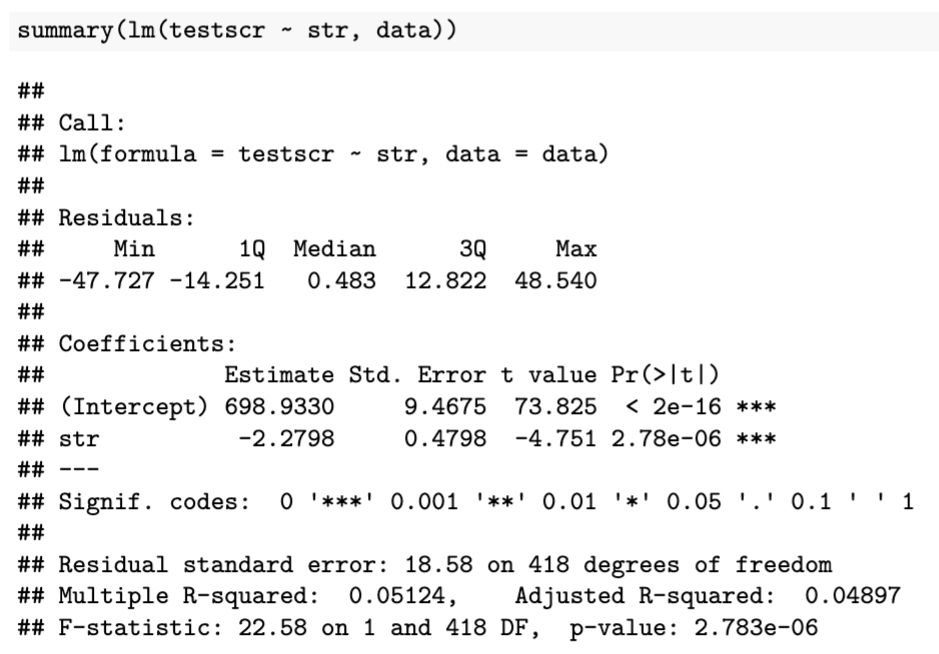
\includegraphics[scale=0.45]{reg_output.png} \\

Let's pay attention to the table below \textit{Coefficients}. This table has two rows, the first row corresponds to the intercept term, and the second row relates to the slope term. We have the coefficients and their corresponding standard errors (or standard deviations) in the second and third columns. While the fourth and fifth columns present the t-value and p-value associated with testing the null hypothesis that the coefficient is 0. Below the table, we also have the value for the $R^2$.   

\newpage

From the output we can see that our estimated model is as follows:
  $$ \hat{wages}_i = 37,681.08 + 587.53 age_i   $$
  
 What does this mean?
 \begin{itemize}
  \item Intercept term, $\hat{\beta_0}=37,681.08$: Average wages for a person of age 0 is \$37,681!
 \item Slope, $\hat{\beta_1}=587.53$: On average, the annual income for individuals who are one year older is \$587.53 higher. Alternatively, we can say that the predicted annual income (according to our model) increases by \$587.53 when age goes up a year. (Avoid attaching a causal interpretation such as age leads to an increase in income etc.)
\end{itemize}

From the output we also see that $R^2 = 0.0214$. This means that age can explain only 2.14\% of the total variation in wages. \\

Note that the interpretation of the slope coefficient is basically how one unit change in the independent variable affects the dependent variable. This can be seen more easily by taking the derivative of $\hat{wages}_i$ with respect to $age_i$\footnote{Refer to the handout on calculus, if your derivatives are a bit rusty.}:

  $$ \frac{\partial \hat{wages}}{\partial age} =  587.53 $$
  
Here $\partial x$ denotes a small change in $x$. \\

Now we have an estimate for the effect of age on wages. But remember, we are still trying to infer something about the population from sample data. In the previous handout, we established that OLS coefficients are unbiased and normally distributed in large samples. This means we can test hypotheses and construct confidence intervals for our coefficients. One hypothesis test that is of most interest is whether the independent variable of interest does not affect our dependent variable. In particular, 
$$ H_0: \beta_1 = 0 \quad \quad \quad H_1: \beta_1 \neq 0  $$

To test this hypothesis we first construct our $t$ statistic (under the null):
$$ t_0 = \frac{\hat{\beta_1}-\beta_1}{S_{\hat{\beta_1}}} = \frac{\hat{\beta_1}}{S_{\hat{\beta_1}}}  $$ 

From the output we know, $\hat{\beta_1} = 587.53 $ and $S_{\hat{\beta_1}}= 22.51$. This implies that our $t$-statistic is $t_0 = 587.53/22.51 = 26.1 $. This $t$-statistic is also reported in the output table (fourth column). We would reject this null at the 5\% level of significance as $t_0=26.1>1.96$. Since we reject the null that age does not affect wages, we can say that age is statistically significant at a 5\% level of significance. \\

The regression output also reports the corresponding $p$-value for $t_0$. Remember, the $p$-value is the percent of outcomes that are more extreme (surprising) than the one we got under the null. So if the null was true, i.e., the effect of age on wages is 0, then what percent of outcomes would be more surprising than getting a coefficient of \$587.53? We can answer this by looking at the $p$-value. Here the $p$-value is pretty close to $0$. We reject the null if the $p$-value is smaller than our significance level. So here, we can reject the null even at a significance level of less than 1\%. \\

 We can construct a 95\% confidence interval for $\beta_1$ as follows:
 
 $$ \hat{\beta_1} \pm 1.96 \times S_{\hat{\beta_1}} = 587.53 \pm 1.96 \times 22.51 = [543.41, 631.64]  $$
 
 We can also use the command \textit{confint} in $R$ after running our regression to to get the confidence intervals. 
 
\begin{lstlisting}
confint(results, level = 0.95)
\end{lstlisting}

\includegraphics[scale=0.65]{cint.png} \\

\newpage

As we saw in class we can use stargazer to produce a prettier looking table. 
\begin{verbatim}
stargazer(results, digits = 2,  type="text", keep.stat=c("n","rsq"))
\end{verbatim}

 I present the output produced by stargazer in Table 1. Output includes the estimated regression coefficients and their standard errors/deviation in the parenthesis. Note, here you can still calculate the t and p-values. In general, you can pick what makes most sense for you to report. \\

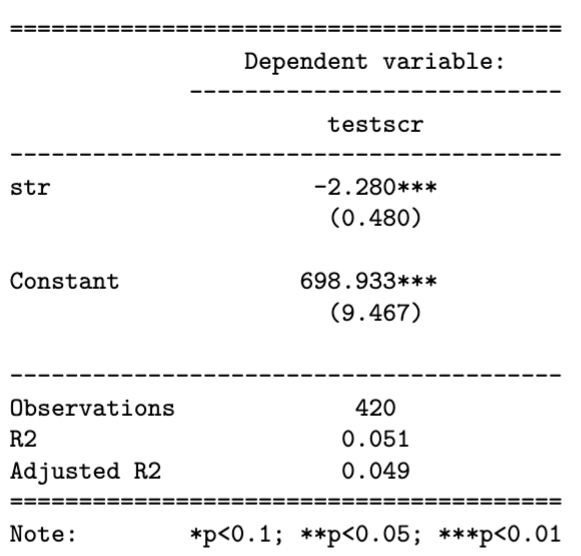
\includegraphics[scale=0.5]{reg_output_stargazer}
 


\end{document}
